\documentclass[12pt,a4paper]{article}

\usepackage[utf8x]{inputenc}

\usepackage{mathpazo}
\usepackage{microtype}
\usepackage{verbatim}
\usepackage{url}

\usepackage{tikz}
\tikzset {>=stealth}

\textwidth=155mm
\textheight=245mm
\topmargin=0pt
\headheight=0pt
\oddsidemargin=0mm
\evensidemargin=0mm
\headsep=0pt
\parindent=0pt
\renewcommand{\baselinestretch}{1.15}
\setlength{\parskip}{0.3\baselineskip plus 1pt minus 1pt}
\addtolength{\jot}{3pt}


\begin{document}
\thispagestyle{empty}

\begin{center}
\textbf{\large An Alternate Method for Solving Quadratic Equations}

\bigskip

\textbf{\large Moti Ben-Ari}

\bigskip

\bigskip

\url{http://www.weizmann.ac.il/sci-tea/benari/}
\end{center}

\begin{footnotesize}
\begin{center}
\copyright{}\ 2020 by Moti Ben-Ari.
\end{center}

This work is licensed under the Creative Commons Attribution-ShareAlike 3.0 Unported License. To view a copy of this license, visit \url{http://creativecommons.org/licenses/by-sa/3.0/} or send a letter to Creative Commons, 444 Castro Street, Suite 900, Mountain View, California, 94041, USA.
\end{footnotesize}

\section{Introduction}

This document presents Po-Shen Loh's alternate method of solving quadratic equations [1, 2]. I have added more examples and details of the computations.

Section~\ref{s.traditional} reviews the traditional methods for solving quadratic equations. Loh's method is based on a very simple observation about the roots that is hard to see intuitively; Section~\ref{s.computing} tries to convince the reader that the observation makes sense and then explains the method for computing roots. In Section~\ref{s.examples} the computation is carried out for two examples. Section~\ref{s.general} derives the traditional formula for the roots from Loh's formulas. Section~\ref{s.irreducible} shows that the method works for polynomials that have complex roots because they are irreducible over the rational numbers. Except for the last Section, the material should be accessible to all secondary-school teachers and students.

\section{Traditional methods for solving quadratic equations}\label{s.traditional}

Every secondary-school student memorizes the formula for obtaining the roots of a quadratic equation $ax^2+bx+c=0$:
\[
x_1, x_2 = \frac{-b\pm\sqrt{b^2-4ac}}{2a}\,.
\]
For now we will work only with monic polynomials; the roots of $x^2+bx+c=0$ are:
\[
x_1, x_2 = \frac{-b\pm\sqrt{b^2-4c}}{2}\,.
\]


Another method of solving quadratic equations is by factoring the polynomials more-or-less by trial and error. Sometimes factoring is very easy:
\begin{eqnarray*}
x^2-4x+3& =& (x-r_1)(x-r_2)=0\\
& =& (x-1)(x-3)=0\\
x_1,x_2&=&1, 3\,.
\end{eqnarray*}
It is much harder to factor:
\[
x^2-2x-24= (x-r_1)(x-r_2)=0\,.
\]
Possible roots $(r_1,r_2)$ are:
\[
(\pm 1,\mp 24)\,, (\pm 2,\mp 12)\,, (\pm 3,\mp 8)\,, (\pm 4,\mp 6)\,.
\]
It is clear that the signs of $r_1,r_2$ must be different so that their product is negative $-24$, but still we have eight possibilities to check.

\section{Computing the roots}\label{s.computing}

\textbf{If $r_1,r_2$ are the roots of $x^2+bx+c$}, then:\footnote{Loh points out the difference between his method and factoring. In the latter, we \emph{assume} that two roots exist. This is true because of the Fundamental Theorem of Algebra, but that is a heavy theorem for the simple task of finding the roots of a quadratic equation. In his method, we simply say: \emph{if the roots exist}.}
\[
(x-r_1)(x-r_2)=x^2 - (r_1+r_2)x + r_1r_2=x^2+bx+c\,.
\]
Even if we do not know the values of the roots, we do know that:
\[
r_1+r_2 = -b\,,\quad\quad r_1r_2=c\,.
\]
Consider some values of $-b,r_1,r_2$ and let $m_{12}$ be the average of $r_1,r_2$:
\[
\renewcommand{\arraystretch}{1.3}
\begin{array}{|r|r|r|r|}
\hline
-b& r_1 & r_2 &m_{12}\\\hline
33 & 12 & 21 & 16\frac{1}{2}\\\hline
33 & 8 & 25 & 16\frac{1}{2}\\\hline
33 & 1 & 32 & 16\frac{1}{2}\\\hline
\hline
-4 & -16 & 12 & -2 \\\hline
-4 & -4 & 0 & -2 \\\hline
-4 & -3 & -1 & -2 \\\hline
\end{array}
\]
For any quadratic equation, the average of the two roots is constant:
\[
\frac{r_1+r_2}{2}=
\frac{(-b-r_2)+r_2}{2}=
\frac{-b}{2}+\frac{-r_2+r_2}{2}=
-\frac{b}{2}\,.
\]
Let $s$ be any number; then:
\[
-b=-b+s+(-s)=\left(\frac{-b}{2}+s\right) + \left(\frac{-b}{2}-s\right)=r_1+r_2\,.
\]
If one root is at distance $s$ from the average $m_{12}$, the other root is at distance $-s$ from  the average:
\[
\renewcommand{\arraystretch}{1.3}
\begin{array}{|r|r|r|r|r|r|}
\hline
-b& r_1 & r_2 & m_{12}& m_{12}-r_1 & m_{12}-r_2\\\hline
33 & 12 & 21 & 16\frac{1}{2}&4\frac{1}{2} & -4\frac{1}{2}  \\\hline
33 & 8 & 25 & 16\frac{1}{2}&8\frac{1}{2}&-8\frac{1}{2}\\\hline
33 & 1 & 32 & 16\frac{1}{2}&15\frac{1}{2}&-15\frac{1}{2}\\\hline
\hline
-4 & -16 & 12 & -2 &14& -14\\\hline
-4 & -4 & 0 & -2&2&-2 \\\hline
-4 & -3 & -1 & -2&1&-1 \\\hline
\end{array}
\]

\bigskip

The following diagram visualizes this relationship for $r_1,r_2=2,6$, where $m_{12}=4, s=2$:
\begin{center}
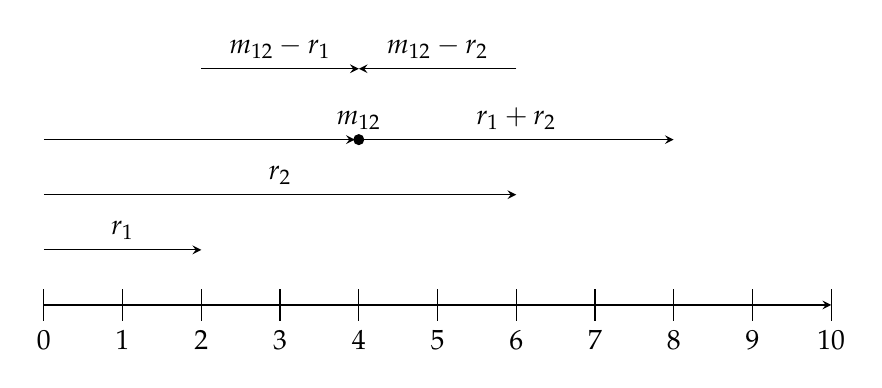
\begin{tikzpicture}
\draw[->] (0,0) -- (10,0);
\foreach \x in {0,1,...,10}
  \draw (\x,-2mm) -- +(0,4mm) node[below,yshift=-4mm] {$\x$};
\draw[->,yshift=7mm] (0,0) -- node[above] {$r_1$} (20mm,0);
\draw[->,yshift=14mm] (0,0) -- node[above] {$r_2$} (60mm,0);
\draw[->,yshift=21mm] (0,0) -- (39.5mm,0);
\draw[->,yshift=21mm] (40mm,0) -- node[above] {$r_1+r_2$} (80mm,0);
\fill (40mm,21mm) circle(2pt) node[above] {$m_{12}$};
\draw[->,yshift=30mm] (20mm,0mm) -- node[above] {$m_{12}-r_1$} +(20mm,0);
\draw[->,yshift=30mm] (60mm,0mm) -- node[above] {$m_{12}-r_2$} +(-20mm,0);
\end{tikzpicture}
\end{center}

If we use other values $r_1,r_2=3,5$ for which $r_1+r_2=8$, $m_{12}=4$ remains the same, while $s=2$ becomes $s=1$:
\begin{center}
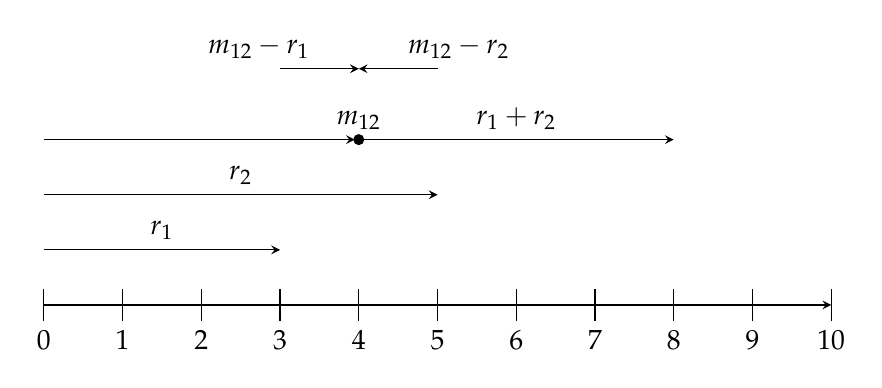
\begin{tikzpicture}
\draw[->] (0,0) -- (10,0);
\foreach \x in {0,1,...,10}
  \draw (\x,-2mm) -- +(0,4mm) node[below,yshift=-4mm] {$\x$};
\draw[->,yshift=7mm] (0,0) -- node[above] {$r_1$} (30mm,0);
\draw[->,yshift=14mm] (0,0) -- node[above] {$r_2$} (50mm,0);
\draw[->,yshift=21mm] (0,0) -- (39.5mm,0);
\draw[->,yshift=21mm] (40mm,0) -- node[above] {$r_1+r_2$} (80mm,0);
\fill (40mm,21mm) circle(2pt) node[above] {$m_{12}$};
\draw[->,yshift=30mm] (30mm,0mm) -- node[above left] {$m_{12}-r_1$} +(10mm,0);
\draw[->,yshift=30mm] (50mm,0mm) -- node[above right] {$m_{12}-r_2$} +(-10mm,0);
\end{tikzpicture}
\end{center}

The offset $s$ seems to be arbitrary in:
\[
r_1=\left(\frac{-b}{2}+s\right)\,,\quad r_2=\left(\frac{-b}{2}-s\right)\,,
\]
but there is an additional constraint $r_1r_2=c$ where $c$ is the constant term in the polynomial. By multiplying the two expressions we have derived for $r_1,r_2$, we can determine $s$ and then $r_1,r_2$.
\[
c=\left(-\frac{b}{2} +s\right)\left(-\frac{b}{2} -s\right)\,.
\]

\section{Examples}\label{s.examples}

Let us use this method on the polynomial  $x^2-2x-24$, where $b=-2,c=-24$:
\begin{eqnarray*}
c&=&\left(-\frac{b}{2} +s\right)\left(-\frac{b}{2} -s\right)\\
-24&=&(1 +s)(1 -s)\\
s^2&=&25\\
s&=&5\\
r_1&=&1+5=6\\
r_2&=&1-5=-4\,.
\end{eqnarray*}

Check:
\[
(x-6)(x-(-4))=x^2-6x-(-4)x+(6\cdot -4)= x^2-2x-24\,.
\]

As another example, let us find the roots of $x^2-83x-2310$:
\begin{eqnarray*}
c&=&\left(-\frac{b}{2} +s\right)\left(-\frac{b}{2} -s\right)\\
-2310&=&\left(\frac{83}{2}+s\right)\left(\frac{83}{2} -s\right)\\
s^2&=&\frac{6889}{4}+2310=\frac{16129}{4}\\
s&=&\frac{127}{2}\\
r_1&=&\frac{83}{2}-\frac{127}{2}=-22\\
r_2&=&\frac{83}{2}+\frac{127}{2}=105\,.
\end{eqnarray*}

Check:
\[
(x+22)(x-105)=x^2+22x-105x+(22\cdot -105)= x^2-83x-2310\,.
\]
Let us compare this computation with the computation using the traditional  formula that we have all memorized:
\begin{eqnarray*}
\frac{-b\pm\sqrt{b^2-4c}}{2}&=&\frac{-(-83)\pm\sqrt{(-83)^2-4\cdot (-2310)}}{2}\\
&=& \frac{83\pm\sqrt{6889+9240}}{2} = \frac{83\pm\sqrt{16129}}{2}\\
&=& \frac{83\pm 127}{2}\\
r_1&=&\frac{83-127}{2}=-22\\
r_2&=&\frac{83+127}{2}=105\,.
\end{eqnarray*}
While the computation in Loh's method is similar to that of the traditional formula, it has the advantage that we can derive it immediately from the average and product of the roots. In the next section, we show that it is easy to derive the traditional formulas from this method.\footnote{See the previous footnote for a theoretical advantage.}

\section{The traditional formula}\label{s.general}

With arbitrary coefficients $b,c$, the equations are:
\begin{eqnarray*}
c=r_1,r_2&=&\left(\frac{-b}{2}+s\right)  \left(\frac{-b}{2}-s\right)\\
&=&\left(\frac{b^2}{4}-s^2\right)\\
s&=&\sqrt{\left(\frac{b^2}{4}\right)-c}\\
r_1,r_2&=&\frac{-b}{2}\pm\sqrt{\left(\frac{b^2}{4}\right)-c}\,,
\end{eqnarray*}
which can also be written:
\[
r_1,r_2=\frac{-b\pm\sqrt{b^2-4c}}{2}\,,
\]
the traditional formula for obtaining the roots of a monic polynomial.

If the polynomial is not monic, $a\neq 1$, divide it by $a$, substitute in the  equation and simplify:
\begin{eqnarray*}
ax^2+bx+c&=&0\\
x^2+\frac{b}{a}x+\frac{c}{a}&=&0\\
r_1,r_2&=&\frac{-(b/a)\pm\sqrt{(b/a)^2-4(c/a)}}{2}\\
&=&\frac{-(b/a)\pm\sqrt{(b/a)^2-4(ac/a^2)}}{2}\\
&=&\frac{-b\pm\sqrt{b^2-4ac}}{2a}\,.
\end{eqnarray*}
The traditional formula has been derived from the observation that $r_1+r_2=-b$ and $r_1r_2=c$.

\section{Irreducible polynomials}\label{s.irreducible}

There are quadratic polynomials like $x^2+1$ that are irreducible over the rational numbers. According to the Fundamental Theorem of Algebra, all polynomials with complex coefficients have complex roots. Let us see how the method works for the polynomial $x^2-2x+76$:
\begin{eqnarray*}
s^2&=&\frac{b^2}{4}-c=\frac{4}{4}-76=-75\\
s&=&\sqrt{-75}=\sqrt{-1\cdot 25\cdot 3}=i\,5\sqrt{3}\\
r_1,r_2&=&1\pm i\,5\sqrt{3}\,.
\end{eqnarray*}
Check:
\[
\renewcommand*{\arraystretch}{1.3}
\begin{array}{ll}
(x-(1+i\,5\sqrt{3}))\;(x-(1-i\,5\sqrt{3}))&=\\
x^2 \,-\, (1+i\,5\sqrt{3})x\,-\,(1-i\,5\sqrt{3})x\,+\,(1^2-(i\,5\sqrt{3})^2)&=\\
x^2 -x -x + 1 - (-75)=\\
x^2-2x+76\,.
\end{array}
\]

\section*{References}

[1] Po-Shen Lo. \textit{A Different Way to Solve Quadratic Equations}, 2019,\\
\url{https://www.poshenloh.com/quadratic/}.

[2] Po-Shen Loh. \textit{A Simple Proof of the Quadratic Formula}, arXiv: 1910.06709, 2019, \url{https://arxiv.org/abs/1910.06709}.

\end{document}
